\documentclass{beamer}

\usepackage{graphicx}
\usepackage{tikz}
\usetikzlibrary{shapes,calc,arrows,chains,decorations.pathmorphing,backgrounds,positioning,fit,scopes}

\setbeamersize{text margin left = 0.2em}
\setbeamersize{text margin right = 0.2em}

\begin{document}

\newcommand{\entry}[1]{\node[entry, on chain]{entry \emph{#1}};}
\newcommand{\deleted}[1]{\node[deleted, on chain]{deleted \emph{#1}};}
\newenvironment{feed}[1]
  {\begin{scope} [start chain=#1,%
                  node distance=0.4ex%
                 ]%
  }
  {\end{scope}}
\newcommand{\feedsbackgrounds}[1]{%
  \begin{pgfonlayer}{background}%
    \foreach \x in {#1} {%
      \node[fit=(\x-begin) (\x-end),feedbackground] (\x-background) {};%
    }%
  \end{pgfonlayer}%
}
\newcommand{\metatext}{\emph{meta:} title, id, author, updated}
\newcommand{\nextlinktext}{\emph{link:} next feed}
\newcommand{\meta}{\node[meta, on chain] {\metatext \\ \nextlinktext };}
\newcommand{\metalast}{\node[meta, on chain] {\metatext \\ (no next link)};}
\newcommand{\nextlink}[2]{%
  \draw[ultra thick,->] (node cs:name=#1-begin,angle=342)%
     to [out=0,in=225] ($(node cs:name=#1-background,anchor=north)!.55!(node cs:name=#2-background,anchor=north)+(0,1em)$)%
     to [out=45,in=90] (node cs:name=#2-background,anchor=north);%
}

\newcommand{\feedspicture}[3]{%
\begin{tikzpicture}[feedspicture]%
  \matrix [feedsmatrix] {%
    \begin{feed}{feeda}%
      \meta #1%
    \end{feed} \pgfmatrixnextcell  %
    \begin{feed}{feedb}%
      \meta #2 %
    \end{feed}   \pgfmatrixnextcell %
    \begin{feed}{feedc}%
      \metalast #3%
    \end{feed} \pgfmatrixendrow %
  };%
%
  \feedsbackgrounds{feeda,feedb,feedc}%
  \nextlink{feeda}{feedb}%
  \nextlink{feedb}{feedc}%
\end{tikzpicture}%
}

\newcommand{\img}[1]{ \includegraphics[width=\textwidth]{images/#1.png} }
\newcommand{\imgopt}[2]{ \includegraphics[#1]{images/#2.png} }

\tikzset{feedspicture/.style={chain default direction=going below},
     feedbackground/.style={fill=orange!100,draw=black!100,inner xsep=0},
     feedelement/.style={
       minimum size=2em,
       minimum width=8em,
       rectangle,
       very thin
     },
     meta/.estyle={feedelement},
     meta/.append style={
       text width=8em,
       align=left,
       outer sep=0
     },
     entry/.estyle={feedelement},
     entry/.append style={
       draw=gray!100,
       fill=lightgray!30,
       font=\itshape
     },
     deleted/.estyle={feedelement},
     deleted/.append style={
       dashed,
       draw=gray!100,
       fill=lightgray!30!red!70,
       font=\itshape
     },
     feedsmatrix/.style={column sep=1.5em}
}

\begin{frame}{Kolab}
  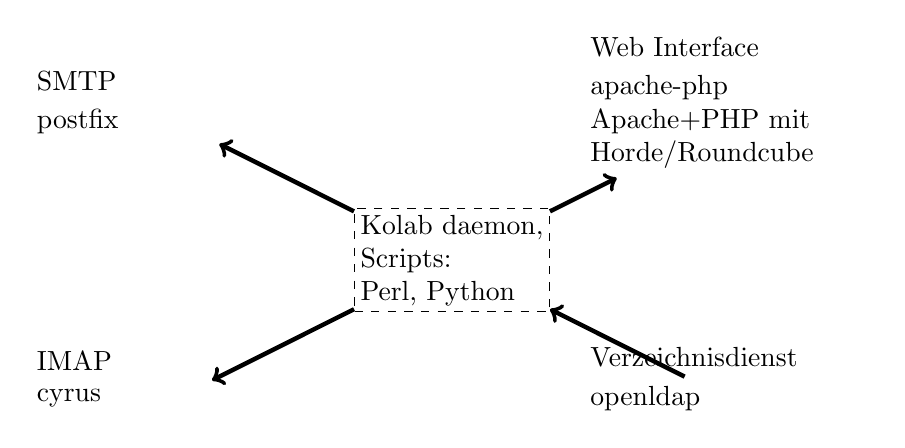
\begin{tikzpicture}[]
    { [every node/.style={text width=10em, node distance=10em}]
      \node (postfix) [label={SMTP}] { \img{postfix} };
      \node (cyrus) [below of=postfix,label={IMAP}] { \img{cyrus} };
      \node (apache) [right of=postfix,label={Web Interface}, node distance=20em] { \img{apache-php} \\ Apache+PHP mit \\ Horde/Roundcube };
      \node (openldap) [below of=apache,label={Verzeichnisdienst}] { \img{openldap} };
    }
    { [every edge/.style={draw,ultra thick}]
    \node [align=left, draw, dashed, inner sep=0.5ex]
       at ($(cyrus)!.5!(apache)$) {Kolab daemon,\\Scripts:\\Perl, Python}
       edge[->] (postfix)
       edge[->] (cyrus)
       edge[->] (apache)
       edge[<-] (openldap);
    }
  \end{tikzpicture}
\end{frame}

\begin{frame}{Kolab clients via connectors}
  \begin{center}
  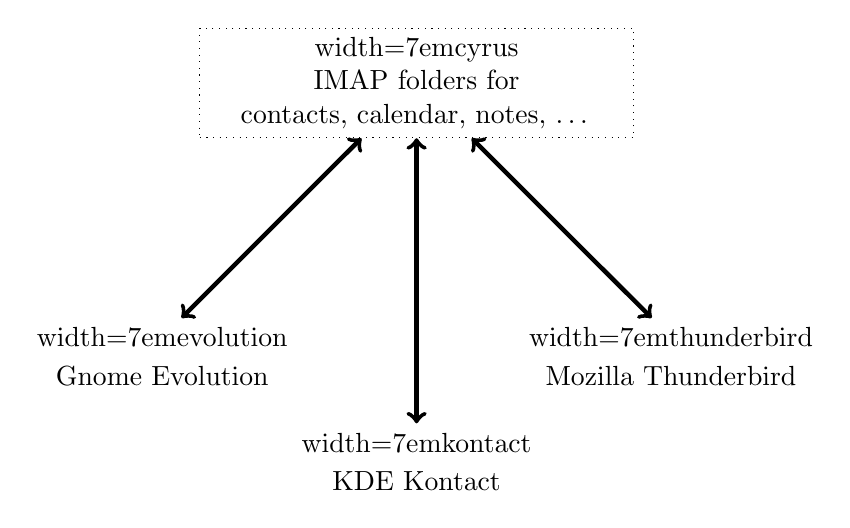
\begin{tikzpicture}
    { [node distance=13em, every edge/.style={draw,ultra thick}]
     \node [text width=15em, align=center, draw, dotted] (cyrus) {\imgopt{width=7em}{cyrus} \\ IMAP folders for \\ contacts, calendar, notes, \ldots};
     \node [below left of=cyrus,label={below:Gnome Evolution}] { \imgopt{width=7em}{evolution}}
       edge[<->] (cyrus) ;
     \node [below of=cyrus,label={below:KDE Kontact}] { \imgopt{width=7em}{kontact}}
       edge[<->] (cyrus) ;
     \node [below right of=cyrus,label={below:Mozilla Thunderbird}] { \imgopt{width=7em}{thunderbird}}
       edge[<->] (cyrus) ;

    }
  \end{tikzpicture}
  \end{center}
\end{frame}


\begin{frame}{Hyperlinks}
  \begin{center}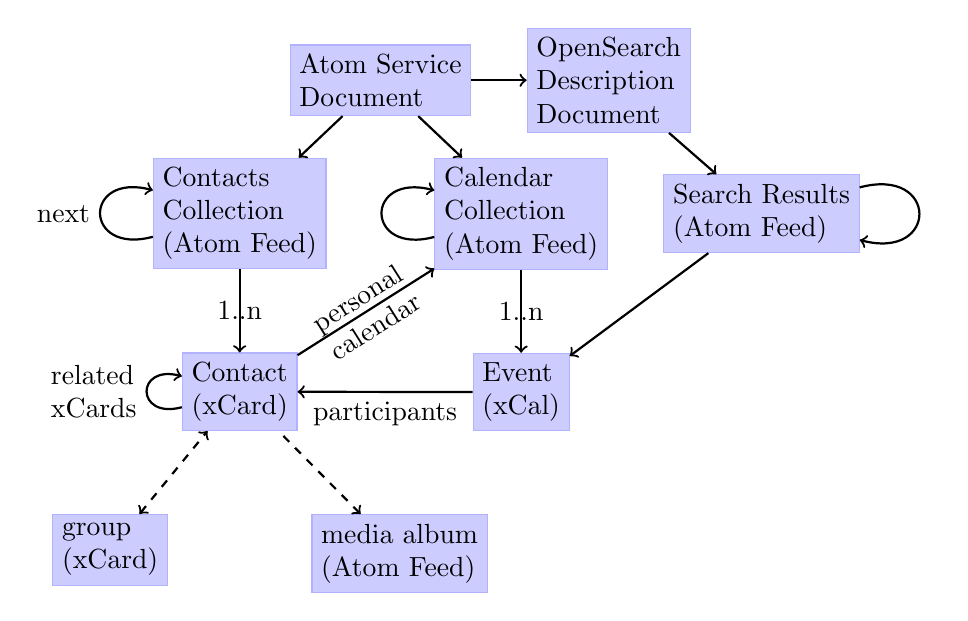
\begin{tikzpicture}[
    align=left,
    every loop/.style={looseness=4},
    every edge/.style={draw, thick},
    doc/.style={rectangle,
                draw=blue!30,fill=blue!20,
                node distance=3em and 0.5em}]
    \node[doc] (svc) [] {Atom Service\\Document};
    \node[doc] (collect) [below left=1.5em and 1.8em of svc,anchor=north] {Contacts\\Collection\\(Atom Feed)}
      edge [<-] node {} (svc)
      edge [->, loop left] node {next} (collect);

    \node[doc] (calcollect) [below right=1.5em and 1.8em of svc,anchor=north] {Calendar\\Collection\\(Atom Feed)}
      edge [<-] node {} (svc)
      edge [->, loop left] node [] {} (calcollect);

    \node[doc] (opensearch) [right=2em of svc] {OpenSearch\\Description\\Document}
      edge [<-] node {} (svc);

    \node[doc] (entry) [below=of collect] {Contact\\(xCard)}
      edge [<-] node {1..n} (collect)
      edge [->] node [sloped] {personal\\calendar} (calcollect)
      edge [->, loop left] node {related\\xCards} (entry);

    \node[doc] (event) [below=of calcollect] {Event\\(xCal)}
      edge [<-] node {1..n} (calcollect)
      edge [->] node [below] {participants} (entry);

    \node[doc] (searchresult) [right=2em of calcollect] {Search Results\\(Atom Feed)}
      edge [->] node {} (event)
      edge [->, loop right] node [] {} (searchresult)
      edge [<-] node {} (opensearch);

    \node[doc] (group) [below left=of entry] {group\\(xCard)}
      edge [<->,style=dashed] node {} (entry);

    \node[doc] (album) [below right=of entry] {media album\\(Atom Feed)}
      edge [<-,style=dashed] node {} (entry);
  \end{tikzpicture}\end{center}
\end{frame}

\begin{frame}[t]{feed after 11 POSTs}
\feedspicture
{ \entry{11} \entry{10} \entry{9} \entry{8} }
{ \entry{7}  \entry{6}  \entry{5} \entry{4} }
{ \entry{3}  \entry{2}  \entry{1} }
\url{http://myapi.org/.../contacts?offset=0|4|8}
\end{frame}

\begin{frame}[t]{POST new entry to feed}
\feedspicture
{ \entry{12} \entry{11} \entry{10} \entry{9} }
{ \entry{8}  \entry{7}  \entry{6}  \entry{5} }
{ \entry{4}  \entry{3}  \entry{2}  \entry{1} }
\end{frame}

\begin{frame}[t]{PUT updated entry 6}
\feedspicture
{ \entry{6} \entry{12} \entry{11} \entry{10} }
{ \entry{9} \entry{8}  \entry{7}  \entry{5} }
{ \entry{4} \entry{3}  \entry{2}  \entry{1} }
\end{frame}

\begin{frame}[t]{DELETE entry 2}
\feedspicture
{ \deleted{2}  \entry{6}  \entry{12} \entry{11} }
{ \entry{10} \entry{9}  \entry{8}  \entry{7} }
{ \entry{5}  \entry{4}  \entry{3}  \entry{1} }
\end{frame}

\begin{frame}[t]{Many more changes}
\feedspicture
{ \entry{7}  \entry{4}  \entry{10} \deleted{11} }
{ \entry{8} \deleted{9}  \entry{1}  \entry{3} }
{ \entry{5}  \entry{12}  \deleted{2}  \entry{6} }
\end{frame}

\begin{frame}[t]{update of entry 6}
\feedspicture
{ \entry{6} \entry{7}  \entry{4}  \entry{10} }
{ \deleted{11} \entry{8} \deleted{9}  \entry{1} }
{ \entry{3} \entry{5}  \entry{12}  }
\end{frame}

\begin{frame}{Execution flow overview}
  \begin{center}
    \includegraphics[width=1\textwidth]{images/executionflowoverview}
  \end{center}
\end{frame}

\begin{frame}{Resource Properties}
\begin{itemize}
\item essential administration properties: unique ID, last update time, HTTP
  entity tag
\item generic meta properties: title, summary, author
\item a media type independent interface corresponding to the concept represented
  by the resource, e.g., a person, location, event, product, \ldots
\item a media type specific serialization (representation) of the resource
\end{itemize}

\end{frame}

\begin{frame}{Facades and their dependencies}
  \begin{center}
    \includegraphics[width=1\textwidth]{images/titleandsummary}
  \end{center}
\end{frame}

\begin{frame}{Facades implementation}
  \begin{center}
    \includegraphics[width=1\textwidth]{images/resourcefacades}
  \end{center}
\end{frame}

\end{document}
